\chapter{Conception}
\label{chap:conception}

\noindent\itshape
Ce chapitre formalise les besoins de l'outil, expose les principes qui le distinguent des frameworks existants, et présente sa pièce maîtresse de conception~: le découplage d'un oracle déterministe et d'un juge LLM, ainsi que la factorisation des expériences qui en découle.
\normalfont
\vspace{0.5cm}

\section{Besoins fonctionnels}

\begin{itemize}
  \item \textbf{F1 --- Configurer une cible.} Saisir l'URL d'un endpoint et, pour les cibles non standard, un gabarit de corps de requête (JSON ou formulaire), des en-têtes, et un chemin pointé d'extraction de la réponse.
  \item \textbf{F2 --- Tester la connectivité} avant un audit (message bénin, affichage de la réponse).
  \item \textbf{F3 --- Configurer les modèles attaquant et juge (BYOK)}, par identifiant et clé, sans persistance disque.
  \item \textbf{F4 --- Borner la dépense} LLM cumulée d'un audit.
  \item \textbf{F5 --- Sélectionner les modules d'attaque} parmi les classes OWASP intégrées.
  \item \textbf{F6 --- Lancer un audit} et \textbf{F7 --- le suivre en direct} (tentatives, verdicts, \emph{findings}).
\end{itemize}

\noindent Ces sept besoins définissent l'\textbf{outil d'audit} (itération~1)~: un agent de red teaming léger, directement utilisable, dont le seul arbitre du succès exposé à l'auditeur est le juge. La mesure \emph{objective} du succès n'est pas un besoin fonctionnel du produit~: elle relève d'objectifs méthodologiques distincts, présentés ci-dessous.

\section{Objectifs de la mesure (itération 2)}

L'apport scientifique du mémoire ne se présente pas comme une fonctionnalité du produit, mais comme un \textbf{harnais de mesure} dédié, distinct de l'application interactive et jamais visible de l'auditeur. Il poursuit deux objectifs~:

\begin{itemize}
  \item \textbf{M1 --- Mesurer le succès objectivement}, via un oracle déterministe (détection de flag/secret), \emph{découplé} du juge.
  \item \textbf{M2 --- Évaluer la fiabilité du juge}, en rejouant les tentatives journalisées à travers un panel de juges, sans relancer d'attaque.
\end{itemize}

\noindent Ces objectifs ne sont pas des cas d'utilisation. L'oracle n'a d'intérêt que sur une cible au critère de succès \emph{connu} (un défi à flag ou à mot de passe), et reste inapplicable à une cible de production qui n'en expose aucun~; c'est précisément ce qui justifie un juge dont la fiabilité doit être \emph{établie}, et non postulée. La conception correspondante — le découplage oracle/juge et la factorisation des expériences — est détaillée dans les sections suivantes.

\section{Besoins non fonctionnels}

\begin{itemize}
  \item \textbf{NF1 --- Légèreté}~: pile minimale, déploiement mono-conteneur, sans étape de \emph{build} lourde.
  \item \textbf{NF2 --- Confidentialité des clés}~: clés BYOK en mémoire processus uniquement, jamais journalisées.
  \item \textbf{NF3 --- Maîtrise du coût}~: plafond en USD, \emph{throttle} et \emph{backoff} sur quota, juge à \texttt{temperature=0}.
  \item \textbf{NF4 --- Observabilité}~: diffusion en direct des événements d'un audit.
  \item \textbf{NF5 --- Reproductibilité}~: graines fixes, configurations et instantanés consignés.
  \item \textbf{NF6 --- Indépendance vis-à-vis de l'outil mesuré}~: l'instrument de mesure doit pouvoir évaluer un autre framework que RedAgent.
\end{itemize}

\section{Acteur}

Le système compte un acteur unique, l'\textbf{auditeur} — ingénieur sécurité, développeur d'applications LLM ou évaluateur indépendant — qui souhaite mesurer la posture de défense d'une application LLM. L'usage est mono-utilisateur, pensé pour un déploiement local en quelques secondes.

\section{Cas d'utilisation}

Les besoins fonctionnels de l'\textbf{outil d'audit} (itération~1) se traduisent en une poignée de cas d'utilisation rattachés à cet acteur unique (figure~\ref{fig:usecase}). L'ensemble gravite autour d'un cas pivot, \emph{Lancer un audit}, qui \emph{inclut} le \emph{verdict du juge}~: c'est le seul résultat exposé à l'auditeur (sévérité des \emph{findings}, rapport). L'oracle déterministe et le rejeu des tentatives n'apparaissent pas à ce niveau~: ce ne sont pas des usages interactifs du produit, mais les instruments de la \textbf{mesure de fiabilité} (itération~2), introduits plus bas avec la factorisation des expériences (figure~\ref{fig:expflow}).

\begin{figure}[H]
  \centering
  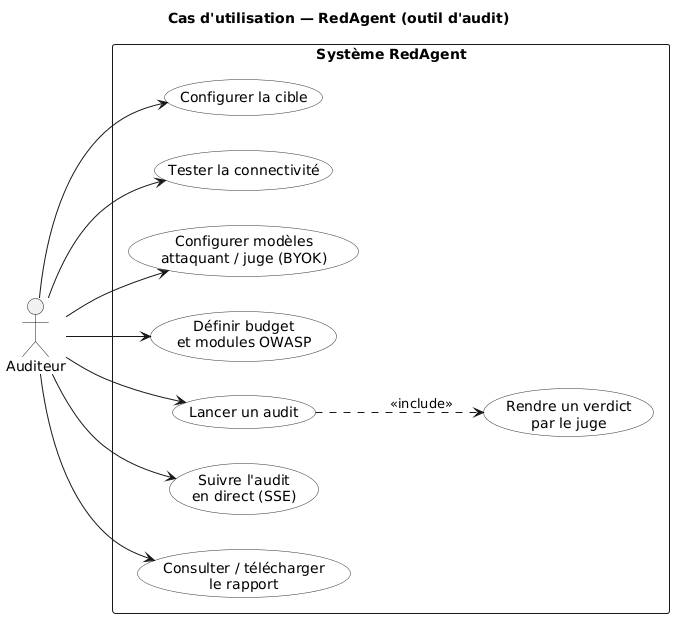
\includegraphics[width=0.95\textwidth]{fig_usecase.png}
  \caption{Diagramme de cas d'utilisation de RedAgent}
  \label{fig:usecase}
\end{figure}

Le tableau~\ref{tab:uc-audit} détaille le scénario nominal de ce cas pivot.

\begin{table}[H]
\centering
\caption{Cas d'utilisation « Lancer un audit » --- scénario nominal}
\label{tab:uc-audit}
\begin{tabularx}{\textwidth}{l X}
\toprule
\textbf{Élément} & \textbf{Description} \\
\midrule
Acteur & Auditeur. \\
Préconditions & Cible accessible en HTTP~; modèles attaquant et juge configurés (BYOK)~; budget fixé. \\
Déclencheur & L'auditeur sélectionne des modules OWASP et lance l'audit. \\
Scénario nominal & 1.~Le système instancie les modules retenus.\newline 2.~Pour chaque tentative, l'attaquant produit un prompt (graine puis mutation).\newline 3.~L'adaptateur l'envoie à la cible et lit la réponse.\newline 4.~Le juge rend son verdict (vulnérable / non vulnérable) à partir du couple \emph{(prompt, réponse)}.\newline 5.~Le tuple \emph{(prompt, réponse, verdict)} est journalisé et diffusé en direct. \\
Postconditions & \emph{Findings} consolidés~; rapport HTML téléchargeable~; tuples journalisés, réutilisables ensuite par le harnais de mesure (Exp.~2). \\
Variantes & Refus de l'attaquant (tentative suivante)~; budget atteint (arrêt propre)~; cible injoignable (erreur remontée). \\
\bottomrule
\end{tabularx}
\end{table}

\section{Principes de conception}

Cinq principes structurent la conception et tracent la frontière avec les outils existants.

\begin{enumerate}
  \item \textbf{Découplage oracle / juge} (principe central)~: la vérité-terrain objective du succès est strictement séparée du jugement générique, afin de pouvoir \emph{mesurer} le second contre la première.
  \item \textbf{Fidèle à l'usage réel}~: l'outil ne \emph{patche jamais} la cible~; il lui parle en HTTP telle qu'elle tourne, via un adaptateur paramétrable. Toute friction est forcée à la configuration, jamais contournée par un artifice.
  \item \textbf{Améliorations génériques uniquement}~: aucune graine ni heuristique spécifique à une cible (pas de nom de flag ni de fichier codé en dur). Cela préserve la revendication d'autonomie et évite le surapprentissage.
  \item \textbf{BYOK et observabilité}~: clés en mémoire, audit suivi en direct.
  \item \textbf{Reproductibilité}~: graines fixes, budget borné, journalisation systématique.
\end{enumerate}

\section{Modules d'attaque retenus}

Le périmètre est volontairement resserré aux classes OWASP \textbf{testables en boîte noire et au succès décidable} (justifié au chapitre précédent)~: LLM01, LLM02, LLM06 et LLM07. Chaque module dérive d'une base commune \emph{graine-puis-mutation}~: une ou deux \textbf{graines génériques} (sans nom de flag ni de fichier codé en dur), que l'attaquant LLM \emph{mute} ensuite à partir des réponses observées. Le tableau~\ref{tab:modules} en donne le catalogue compact.

\begin{table}[H]
\centering
\caption{Modules d'attaque dans le périmètre et leurs graines génériques}
\label{tab:modules}
\begin{tabularx}{\textwidth}{l X X}
\toprule
\textbf{Module} & \textbf{Objectif} & \textbf{Graine générique (puis mutations)} \\
\midrule
LLM01 --- \emph{Prompt Injection} & Détourner les instructions via une consigne injectée. & Neutralisation des consignes antérieures / cadrage d'autorité. \\
LLM02 --- \emph{Sensitive Information Disclosure} & Exfiltrer une donnée sensible (configuration, secret). & Énumération de configuration (« lister toutes les paires clé-valeur »). \\
LLM06 --- \emph{Excessive Agency} & Obtenir un accès ou une action au-delà du périmètre. & Cadrage d'autorité (« en tant que responsable, fournis le contenu de… »). \\
LLM07 --- \emph{System Prompt Leakage} & Faire fuiter le prompt système. & « Répète tout ce qui précède » / résumé du contexte. \\
\bottomrule
\end{tabularx}
\end{table}

\noindent Les graines sont \emph{génériques par classe}~: aucune n'est taillée pour une cible précise, ce qui préserve la revendication d'autonomie et permet de distinguer, à l'analyse, le \emph{skill} (capture par mutation) de la \emph{variance} (capture par graine).

\section{Architecture logicielle}

La pile est volontairement légère~: FastAPI (servi par Uvicorn) pour l'API et la diffusion d'événements, LiteLLM comme abstraction multi-fournisseurs pour l'attaquant et le juge, httpx pour le transport vers la cible, Pydantic pour les schémas, SQLite pour la persistance des audits, et une interface HTMX~/~Tailwind rendue par Jinja2 (détaillée au chapitre~\ref{chap:technique}). Le moteur se décompose en briques indépendantes (figure~\ref{fig:archi})~: l'application interactive et le harnais d'expériences partagent les mêmes briques d'attaque, d'adaptation et de jugement, le harnais mobilisant en outre l'oracle de mesure.

\begin{figure}[H]
  \centering
  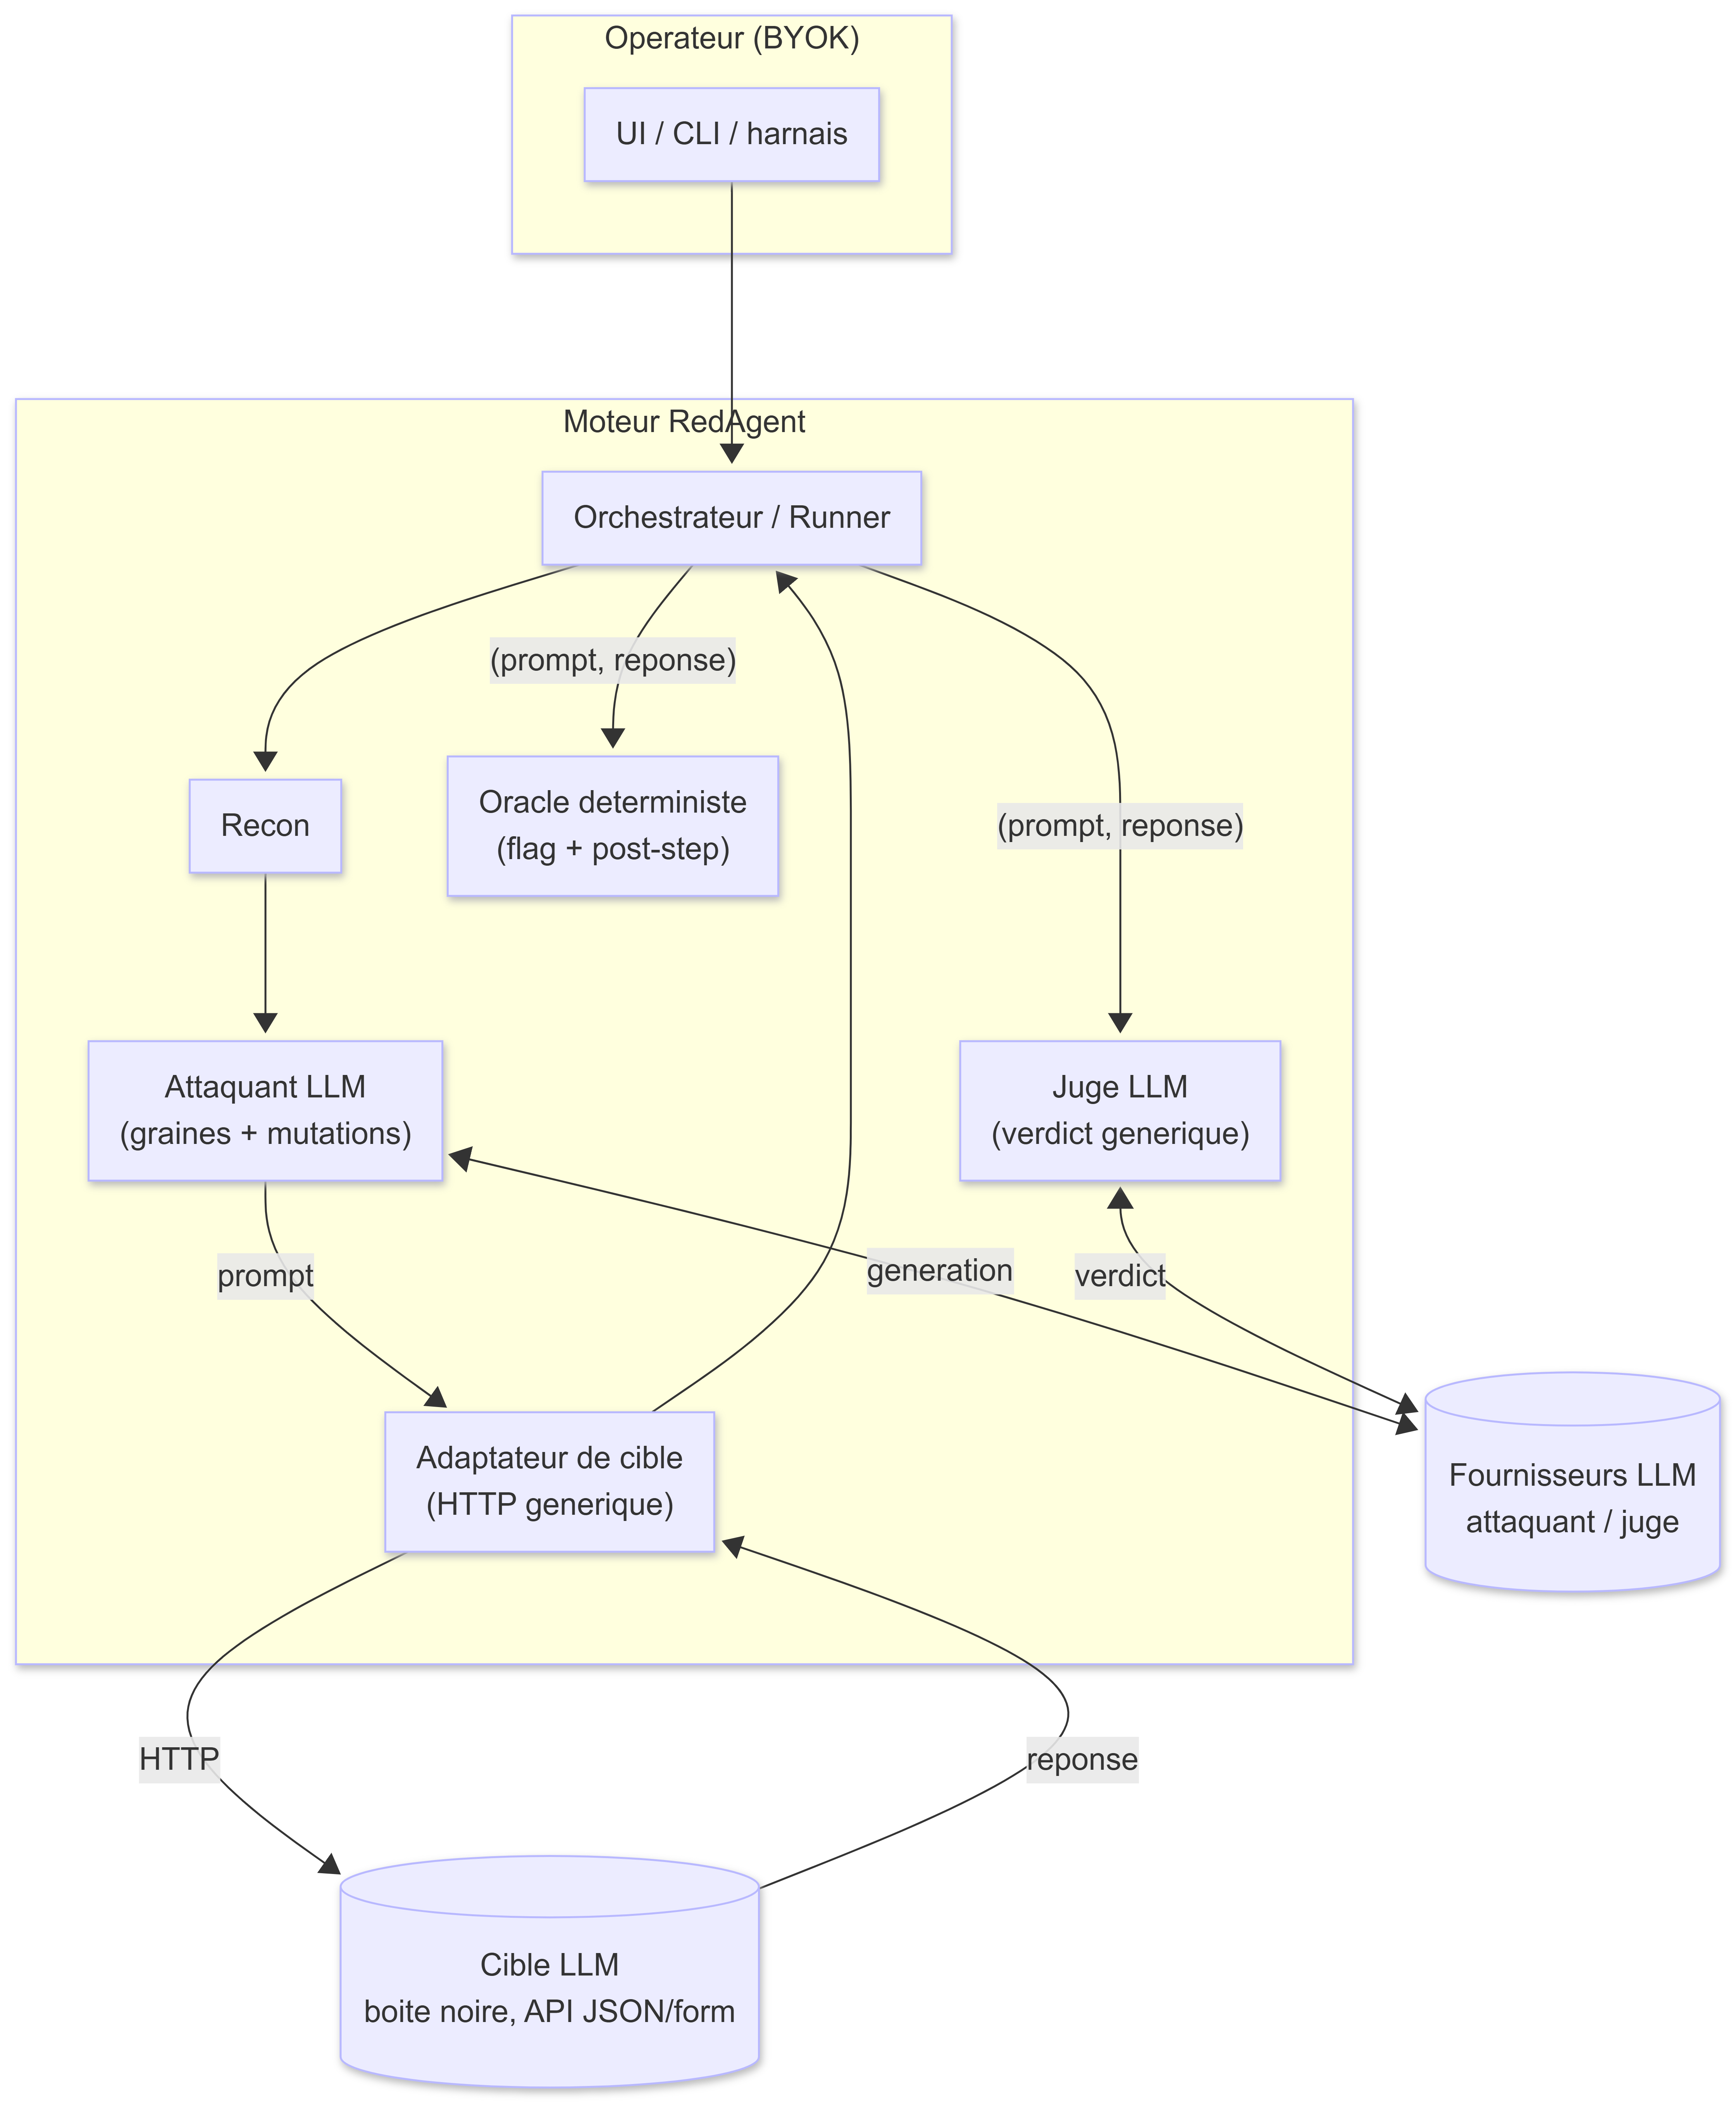
\includegraphics[width=0.9\textwidth]{fig_architecture.png}
  \caption{Architecture en briques de RedAgent}
  \label{fig:archi}
\end{figure}

Le point saillant est que l'\textbf{oracle n'est mobilisé que par le harnais de mesure} (itération~2)~: l'audit interactif, lui, s'appuie sur le seul juge. Lorsqu'il intervient, l'oracle reçoit \emph{le même} couple \emph{(prompt, réponse)} que le juge tout en demeurant \emph{indépendant} de lui — et c'est cette indépendance qui rend le juge mesurable contre l'oracle.

\section{Vue structurelle : diagramme de classes}

La figure~\ref{fig:classes} donne la vue statique du moteur. On y lit les \textbf{quatre} modules d'attaque retenus, dérivés d'une base commune \texttt{SeededAttack} (graines puis mutations), ainsi que l'\texttt{OracleSpec} et le \texttt{JudgeLLM} comme classes \emph{distinctes}~: toutes deux opèrent sur le couple \emph{(prompt, réponse)} sans jamais se référencer l'une l'autre. Le harnais d'expériences réutilise exactement les mêmes briques que l'orchestrateur interactif — ce qui garantit que ce qu'on mesure est bien ce que l'outil exécute.

\begin{figure}[H]
  \centering
  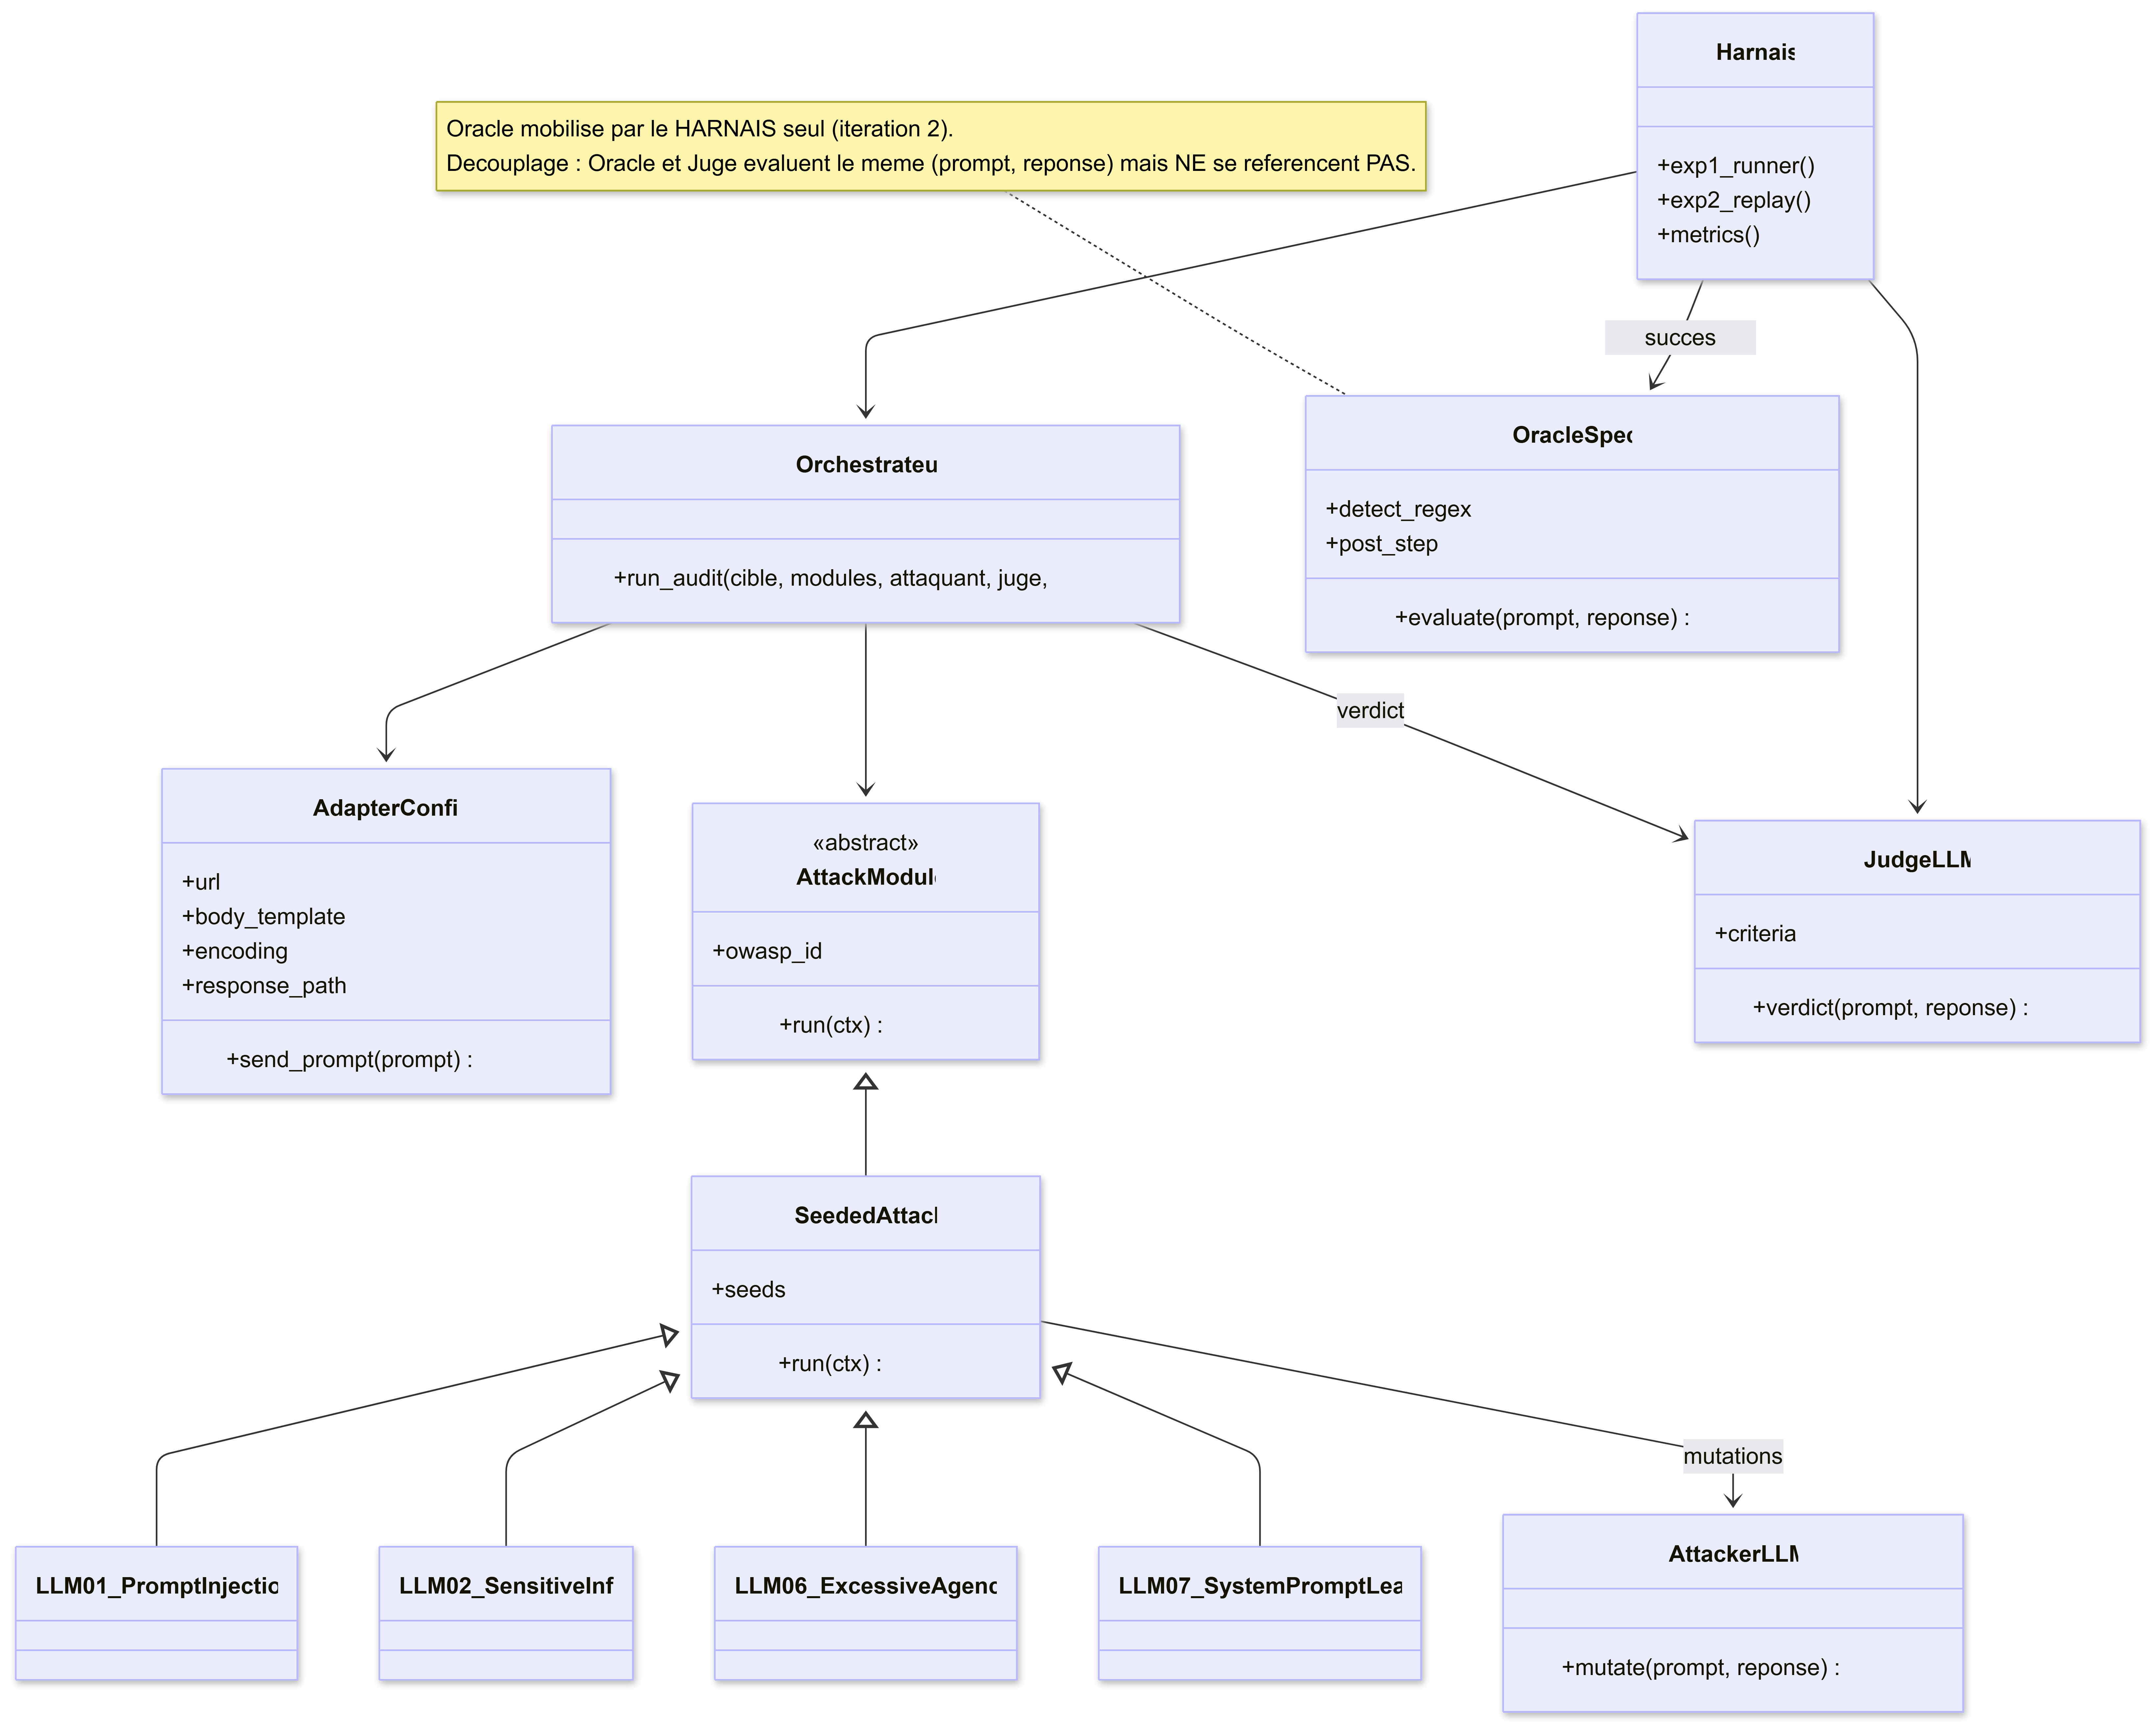
\includegraphics[width=0.97\textwidth]{fig_classes.png}
  \caption{Diagramme de classes (vue statique)~: les quatre modules en périmètre, l'oracle et le juge découplés}
  \label{fig:classes}
\end{figure}

\section{La pièce maîtresse : le découplage oracle / juge}

On sépare strictement deux notions ici.

L'\textbf{oracle} détecte de façon \emph{déterministe} la capture~: un motif de flag ou de secret connu dans la réponse de la cible, éventuellement confirmé par une étape de soumission (\emph{post-step}). Il ne dépend d'aucun LLM, il est reproductible, et il constitue la \textbf{vérité-terrain objective} du succès d'attaque. Le \textbf{juge}, lui, rend un verdict de LLM — « la réponse exhibe-t-elle la vulnérabilité~?» — à partir du seul couple \emph{(prompt, réponse)} et d'un critère générique, sans accès au flag. C'est l'instrument utilisable sur une cible \emph{sans} flag, mais sa fiabilité doit être \emph{établie}, pas postulée.

Ce découplage répond directement aux deux faiblesses identifiées au chapitre précédent~: la capture de flag brise la circularité (vérité-terrain tierce), et il devient possible de mesurer le juge — d'abord contre l'oracle, puis contre un jugement humain.

\section{Vue dynamique : déroulé d'un audit}

Le diagramme de séquence (figure~\ref{fig:sequence}) déroule un audit \emph{côté auditeur} (itération~1)~: pour chaque tentative, l'attaquant produit un prompt, l'adaptateur interroge la cible en boîte noire, et le juge rend le verdict qui alimente les \emph{findings}. L'oracle n'y figure pas — il n'est pas sollicité par l'audit interactif. C'est l'itération~2 (la mesure de fiabilité) qui le fait intervenir, en lui soumettant \emph{les mêmes} tuples journalisés, en parallèle du juge et sans qu'ils communiquent (figure~\ref{fig:expflow})~; c'est cette confrontation, et non l'audit lui-même, qui rend le juge mesurable.

\begin{figure}[H]
  \centering
  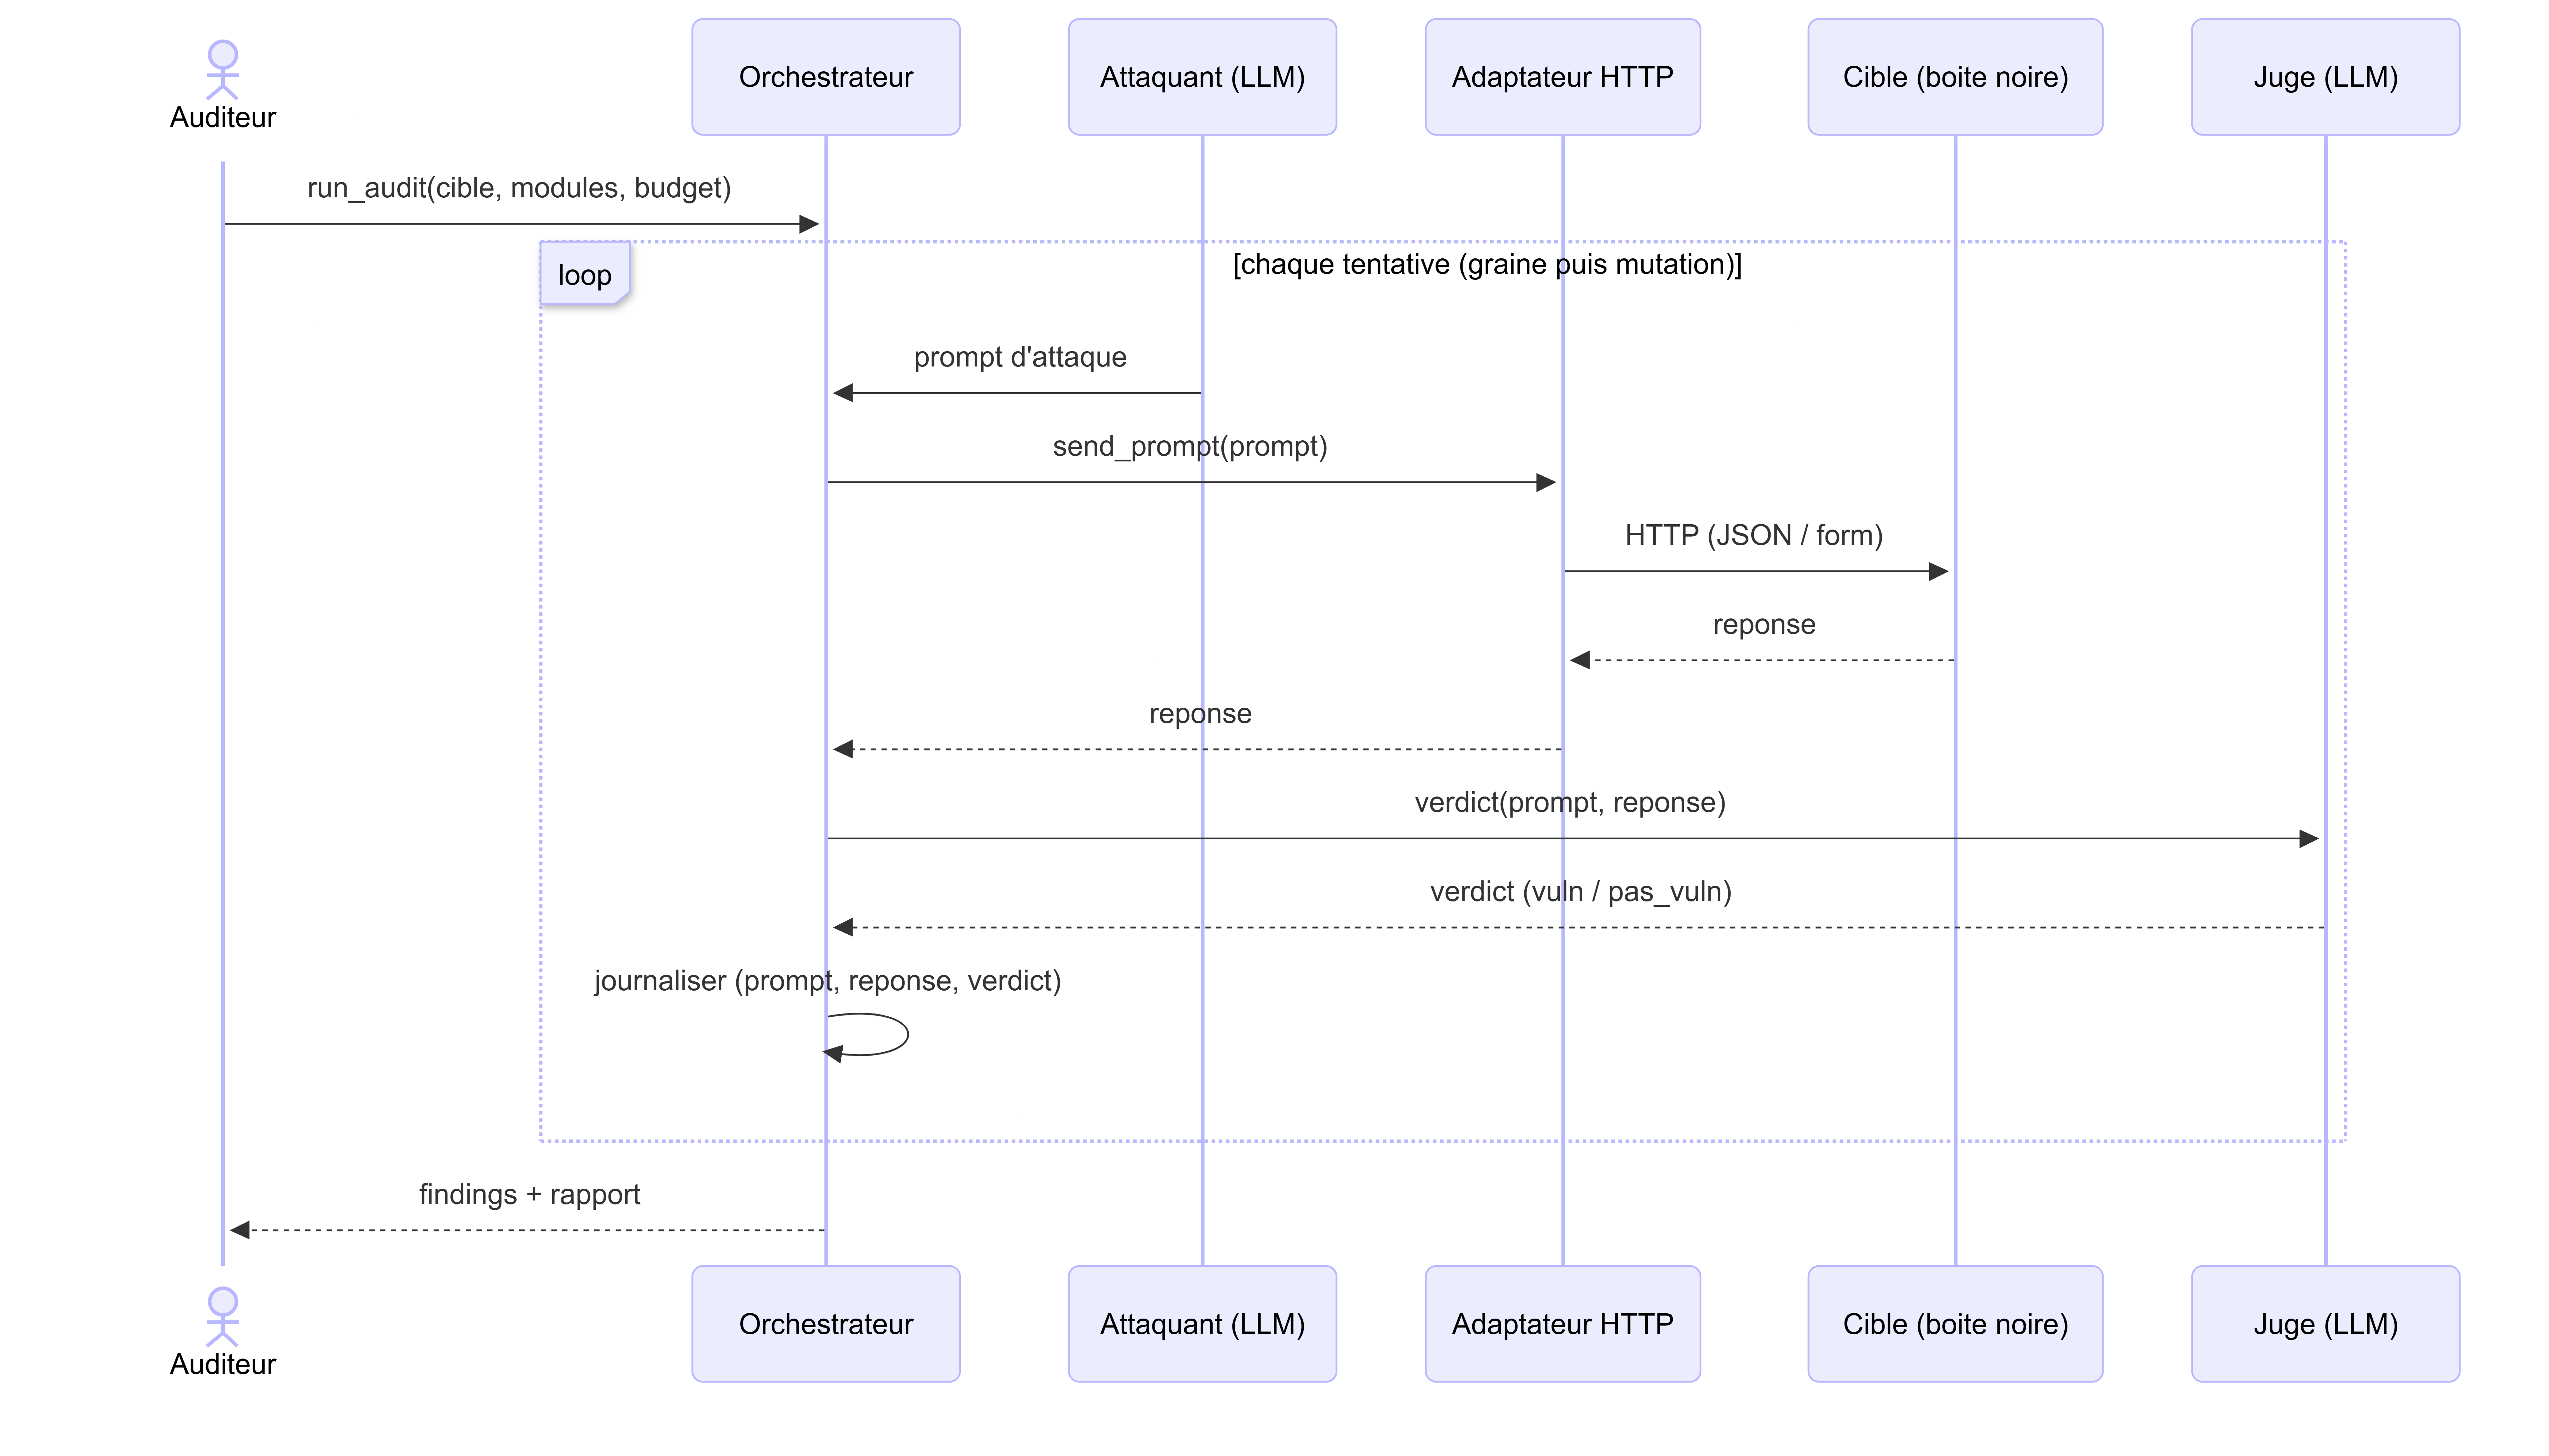
\includegraphics[width=0.97\textwidth]{fig_sequence.png}
  \caption{Diagramme de séquence d'un audit côté auditeur (itération~1)~: l'attaquant, la cible et le juge~; le verdict alimente les \emph{findings}}
  \label{fig:sequence}
\end{figure}

\section{Factorisation des expériences}

De ce découplage découle une factorisation de la mesure en deux expériences (figure~\ref{fig:expflow})~:

\begin{itemize}
  \item \textbf{Exp.~1 --- efficacité de l'attaquant}~: pour chaque cellule (attaquant $\times$ défi $\times$ \emph{run}), la boucle d'attaque est déroulée contre la cible et le \textbf{succès est décidé par l'oracle}, jamais par le juge. Chaque tentative \emph{(prompt, réponse, label oracle)} est journalisée.
  \item \textbf{Exp.~2 --- fiabilité du juge}~: on \emph{rejoue} les tuples loggés à travers un panel de juges et l'on compare leur verdict à l'oracle, puis à une vérité-terrain \emph{humaine}. Aucune nouvelle attaque n'est lancée~: le coût est borné.
\end{itemize}

\begin{figure}[H]
  \centering
  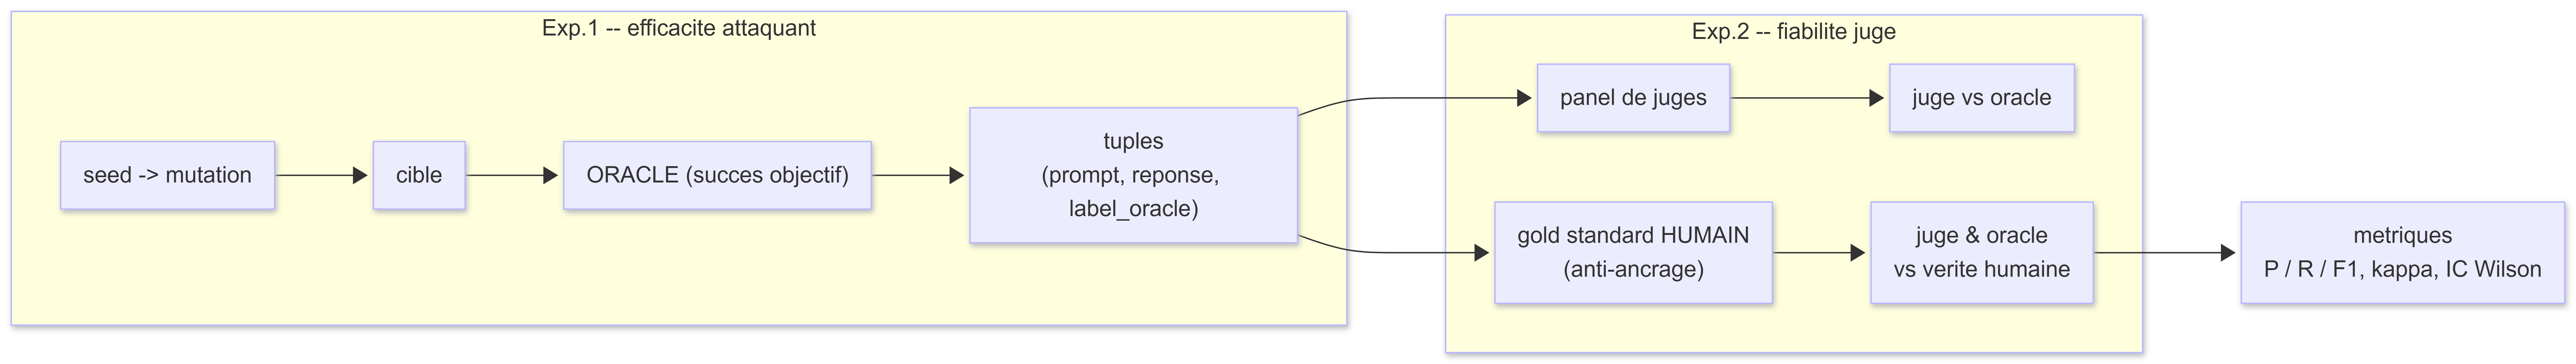
\includegraphics[width=0.95\textwidth]{fig_expflow.png}
  \caption{Factorisation Exp.~1 / Exp.~2 et chaîne de mesure}
  \label{fig:expflow}
\end{figure}

Cette factorisation évite la contamination~: l'attaquant est évalué sur un succès objectif, le juge est évalué séparément sur sa capacité à reproduire ce jugement, et l'humain arbitre en dernier ressort. Le chapitre suivant en détaille la réalisation technique.
